58. а) $y=\cfrac{2(x-1)}{3x-2-x^2}=\cfrac{2(x-1)}{-(x-1)(x-2)}=\cfrac{2}{2-x},\ x\neq1.$
$$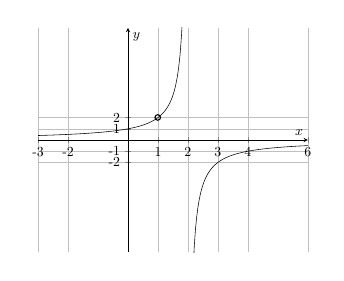
\begin{tikzpicture}[scale=0.5]
\begin{axis}[
    axis lines = middle,
    grid=major,
    legend pos={south west},
    xlabel = {$x$},
    %xlabel style={below right},
    ylabel = {$y$},
    ymin=-10,
    ymax=10,
    xmin=-3,
    xmax=6,
    xtick={-2,-3,1,2,3,4,6},
    xticklabels={-2,-3,1,2,3,4,6},
    ytick={-2,-1,1,2},
    yticklabels={-2,-1,1,2},
                  ]
	\addplot[domain=-3:1.99, samples=100, color=black] {2/(2-x)};
    \addplot[domain=2.01:6, samples=100, color=black] {2/(2-x)};
   % \addplot[domain=-3:3, samples=100, color=black] {-x};
     %\addlegendentry{$\text{Рис. 1}$};
\end{axis}
\draw (3.04,3.42) circle (2pt);
\end{tikzpicture}$$
б) По графику определим количество решений: $a\in\left\{0;2\right\}:0,\ a\in(-\infty;0)\cup\left(0;2\right)\cup\left(2;+\infty\right):1.$\\
